\RequirePackage[OT1]{fontenc}
\documentclass[conference]{IEEEtran}
\IEEEoverridecommandlockouts
% The preceding line is only needed to identify funding in the first footnote.
% If that is unneeded, please comment it out.

\usepackage{cite}
\usepackage{amsmath,amssymb,amsfonts}
\usepackage{algorithmic}
\usepackage{algorithm}
\usepackage{graphicx}
\usepackage{textcomp}
\usepackage{xcolor}
\usepackage{tabularx}
\usepackage{float}
\usepackage{caption}
\usepackage{booktabs}
\newcommand{\ieeeemph}[1]{\textbf{#1}}

\usepackage{verbatim}

\usepackage[numbers,sort&compress]{natbib}
\usepackage{marvosym}
\usepackage{bm}
\usepackage{float}
\usepackage{multirow}
\usepackage{stfloats}
\usepackage{hyperref}
\usepackage[utf8]{inputenc}

\newtheorem{owndefinition}{Definition}

\def\sm{\smallskip}

\ifCLASSINFOpdf

\else
\fi

\def\BibTeX{{\rm B\kern-.05em{\sc i\kern-.025em b}\kern-.08em
    T\kern-.1667em\lower.7ex\hbox{E}\kern-.125emX}}

\begin{document}

\title{LLM-Based Semantic Extraction for Design-Time Business Process Compliance Checking}

\author{
\IEEEauthorblockN{
Yingchao Huo\textsuperscript{},
Xiaoqing Chen\textsuperscript{},
Jiahao Ma\textsuperscript{},
Guosheng Kang\textsuperscript{\Letter},
Wen Li\textsuperscript{},
Jiayan Xiang\textsuperscript{}
}
\IEEEauthorblockA{
\textsuperscript{1}Hunan Provincial Key Lab. for Services Computing and Novel Software Technology, HNUST, Xiangtan, Hunan, China\\
\textsuperscript{2}School of Computer Science and Engineering, Hunan University of Science and Technology, Xiangtan, China\\
Email: \{huoyingchao666, xiaoqingchen696, jiahaoma2627, guoshengkang, wenli0023cs, jiayanxiang02\}@gmail.com
}
}

\maketitle

\begin{abstract}
Business process compliance (BPC) checking aims to determine whether business processes conform to regulatory requirements and is an important task in business process management. Existing approaches typically transform natural-language regulations into structured representations for subsequent compliance checking. However, semantic extraction in this process often relies on manually designed rules or lexical resources, which requires considerable human effort and may have difficulty handling diverse regulatory expressions. To address this issue, we introduce LLM-based Semantic Extraction (LLM-SE) into a three-part design-time BPC checking framework. Given regulatory requirements, LLM-SE extracts six types of regulatory semantics, including modality, actor, action, condition, constraint, and exception. A deterministic post-processing procedure further performs structural adaptation, evidence alignment, and validation to construct structured Rule Records. 
The resulting Rule Records are combined with Process Records derived from BPMN models in Part 3, which follows the matching and three violation definitions of Sun et al.
 Experiments on regulatory requirements and process models demonstrate the effectiveness of the proposed approach.
\end{abstract}

\begin{IEEEkeywords}
Business Process Compliance, Design-Time Compliance Checking, Large Language Models, Compliance Requirement Parsing, Semantic Extraction
\end{IEEEkeywords}

\section{Introduction}
\label{sec:1}

Business process compliance (BPC) aims to ensure that business processes conform to laws, regulations, standards, and organizational policies~\cite{hashmi2018we}. Design-time compliance checking identifies potential violations before execution, reducing non-compliance risks and costs. A key challenge is the semantic gap between natural-language regulatory requirements and the activities, responsibilities, and control-flow structures of process models. Existing studies have explored compliance rule representations to support automated checking~\cite{zasada2023evaluation}.

Early BPC studies used structured compliance representations. Awad et al.~\cite{awad2008efficient} combined BPMN-Q with temporal logic, Elgammal et al.~\cite{elgammal2016formalizing} introduced compliance patterns, and Governatori et al.~\cite{governatori2016semantic} used LegalRuleML for compliance checking. Such representations still need to be derived from regulatory documents. Sleimi et al.~\cite{sleimi2018automated} extracted semantic legal metadata using natural language processing, while Michel et al.~\cite{michel2022identification} identified decision rules from legislation. Winter et al.~\cite{winter2020assessing} assessed process models against regulatory documents. Sun et al.~\cite{sun2024design} proposed a multi-granularity approach that extracts six regulatory semantics---modality, actor, action, condition, constraint, and exception---for violation detection using process-model information. Their approach reduces manual formalization but still relies on predefined linguistic patterns and lexical resources for semantic extraction.

Large language models (LLMs) have also been applied to regulatory analysis. De Kinderen and Winter~\cite{de2024towards} studied prompt-based generation of legal requirement models. Barrientos et al.~\cite{barrientos2026impact} combined LLM-based and algorithmic methods to analyze the impact of regulatory changes on BPC, and later studied legal-change management~\cite{barrientos2026taming}. Guliani et al.~\cite{guliani2026dejure} proposed De Jure, an iterative LLM-based pipeline for structured regulatory rule extraction. For process-related tasks, Wang et al.~\cite{wang2025leveraging} used LLM-generated process information for compliance risk identification, Park et al.~\cite{park2026extracting} extracted Declare constraints from natural-language process descriptions, and K\"olbel et al.~\cite{koelbel2026context} combined BPMN models with external security knowledge using LLMs for process explanation and compliance assessment.

However, these studies differ in their representations and checking tasks. We therefore investigate two questions: whether LLMs can extract the semantics required by an existing design-time BPC framework more accurately than a conventional extractor under the same fine-grained representation and evaluation procedure, and how the resulting Rule Records affect downstream compliance checking.

We investigate LLM-SE within a three-part design-time BPC framework: Process Model Parsing, Compliance Requirement Parsing, and Compliance Checking. The first two parts independently transform BPMN models and natural-language requirements into Process Records and Rule Records, respectively. Our contribution focuses on Compliance Requirement Parsing, where LLM-SE extracts regulatory semantics and deterministic post-processing constructs valid Rule Records. Compliance Checking combines both records for rule--process matching and detection of missing-action, incorrect-actor, and out-of-order violations.

The main contributions of this work are:
\begin{itemize}
    \item We propose LLM-based Semantic Extraction (LLM-SE) for compliance requirement parsing. It extracts six regulatory semantic elements---modality, actor, action, condition, constraint, and exception---and constructs structured Rule Records for compliance checking.

    \item We design a modular prompt combining task and schema specifications with semantic examples, semantic guidance, and output-discipline instructions. We also develop deterministic post-processing that performs structural adaptation, evidence alignment, relation cleanup, and validation to convert raw LLM outputs into valid Rule Records.

    \item We evaluate LLM-SE against an independently reconstructed Rules-Only baseline under the same semantic representation and evaluation procedure. We further analyze prompt components and examine how the resulting Rule Records affect compliance checking for three violation types.
\end{itemize}

\begin{figure*}[!t]
    \centering
    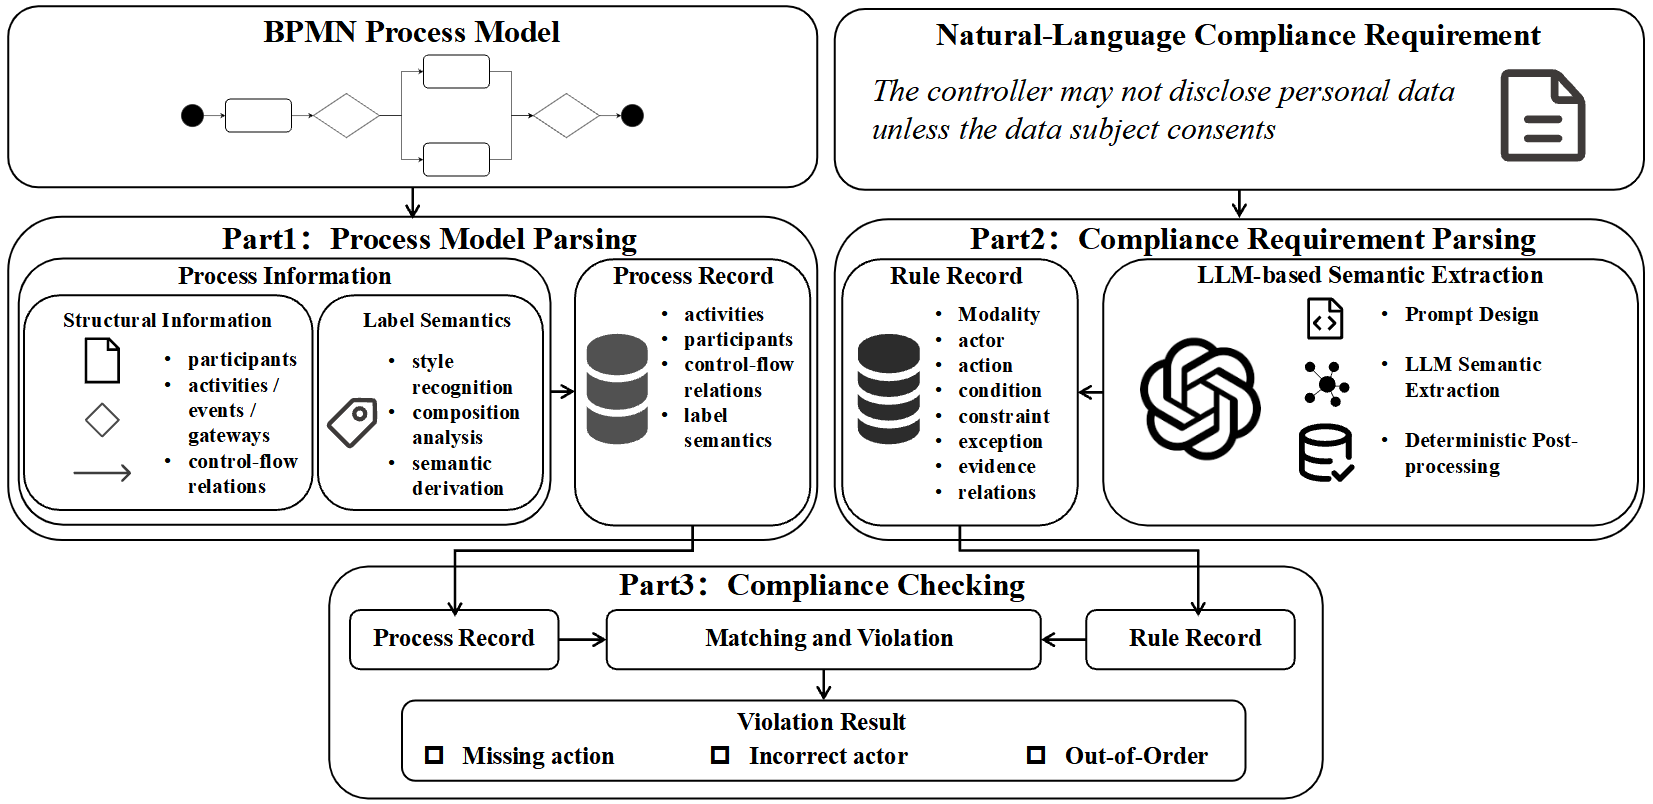
\includegraphics[width=0.90\textwidth,keepaspectratio]{fig1.png}
    \caption{Overall framework for design-time business process compliance checking.}
    \label{fig:framework}
\end{figure*}

\section{Problem Formulation and Framework}
\label{sec:2}

\subsection{Problem Formulation}
\label{sec:2.1}

Following the design-time BPC setting of Sun et al.~\cite{sun2024design}, we aim to identify potential violations of natural-language compliance requirements in BPMN process models before execution.

A BPMN model is transformed into a Process Record containing process elements, participants, and control-flow relations, with actors, actions, and business objects derived from process labels and associated with their activities. A compliance requirement is transformed into a Rule Record containing six regulatory semantic elements: modality, actor, action, condition, constraint, and exception.

Following Sun et al.~\cite{sun2024design}, modality specifies the normative type, such as obligation, prohibition, or permission. Actor identifies the responsible entity, and action describes the required behavior. Condition specifies when a requirement applies, constraint describes restrictions on its applicability, and exception specifies when it does not apply. The Rule Record also preserves supporting textual evidence and relations between elements.

The two records support rule--process matching and checking for three violation types: missing action, incorrect actor, and out-of-order execution.

\subsection{Overall Framework}
\label{sec:2.2}

As shown in Fig.~1, Process Model Parsing extracts structures, control-flow relations, and label semantics from BPMN models to form Process Records. Independently, Compliance Requirement Parsing uses LLM-SE and deterministic post-processing to construct valid Rule Records from natural-language requirements. Compliance Checking combines both records for rule--process matching and detection of missing-action, incorrect-actor, and out-of-order violations.

\begin{figure*}[!t]
    \centering
    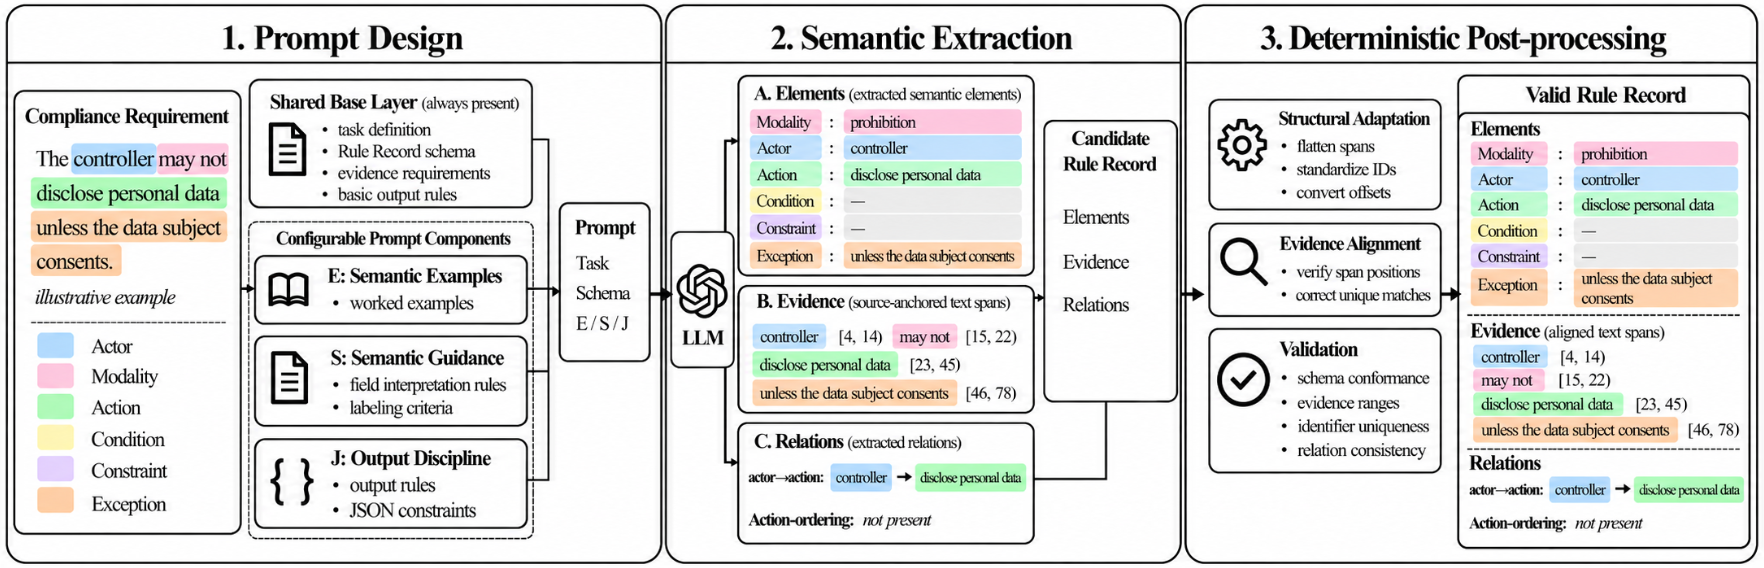
\includegraphics[width=0.98\textwidth,keepaspectratio]{fig2.png}
    \caption{Detailed workflow of LLM-based semantic extraction.}
    \label{fig:part2}
\end{figure*}

\section{Methodology}
\label{sec:3}

\subsection{Process Model Parsing}
\label{sec:3.1}

Following Sun et al.~\cite{sun2024design}, we extract structural and semantic information from BPMN models. A deterministic parser identifies activities, events, gateways, pools, lanes, sequence flows, and their labels. Control-flow relations, including direct connections, reachability, and activity ordering, are derived from sequence flows.

Actors are identified from process context, such as pools and lanes. Following Sun et al., activity labels undergo label style recognition, label composition analysis, and semantic content derivation to identify actions and business objects. The resulting Process Record contains structural information and associates extracted label semantics with their corresponding activities for compliance checking.

\subsection{Compliance Requirement Parsing}
\label{sec:3.2}

Unlike Sun et al.~\cite{sun2024design}, whose semantic extraction relies on predefined linguistic patterns and lexical resources, our LLM-based Semantic Extraction (LLM-SE) uses prompt-guided extraction to identify regulatory semantics from natural-language requirements. We retain the same six semantic categories---modality, actor, action, condition, constraint, and exception---for comparison under a common representation. As shown in Fig.~\ref{fig:part2}, LLM-SE consists of three steps: Prompt Design, Semantic Extraction, and Deterministic Post-processing.

\textbf{Prompt Design.} We design a modular prompt with a fixed shared base layer and three configurable components. The base layer defines the extraction task, target Rule Record schema, evidence requirements, and basic output rules. Component \(E\) provides worked examples, \(S\) provides detailed semantic guidance, and \(J\) adds JSON formatting and output-discipline instructions. This design separates essential extraction requirements from optional guidance, allowing the effects of \(E\), \(S\), and \(J\) to be evaluated independently without changing the basic task or output structure.

\textbf{LLM-based Semantic Extraction.} Given a compliance requirement and the designed prompt, the LLM extracts semantic elements, supporting textual evidence, and relations between elements in a single call. The output forms a candidate Rule Record in JSON format, with source-anchored evidence spans and element identifiers for actor--action and ordering relations. For example, from ``The controller may not disclose personal data unless the data subject consents,'' the model identifies ``controller'' as the actor, ``disclose personal data'' as the action, and ``unless the data subject consents'' as an exception. Unlike the Rules-Only baseline, LLM-SE does not use predefined linguistic extraction patterns or baseline predictions to identify these elements.

\textbf{Deterministic Post-processing.} Following the use of structured outputs and schema validation in regulatory analysis~\cite{barrientos2026impact}, we apply deterministic processing to adapt and validate the generated Rule Record. Structural adaptation converts supported output formats into the target schema by flattening nested spans, standardizing identifiers, converting valid numeric strings into integer offsets, and generating normalized values from the extracted text.

Evidence alignment checks whether each extracted span matches its recorded source position. Character offsets use zero-based start and exclusive end positions. Correct coordinates are retained; otherwise, the procedure searches for an exact text match within the corresponding source clause. A unique match allows coordinate correction, while unmatched or ambiguous spans are removed. For example, if ``disclose'' is extracted with incorrect offsets but occurs only once in the clause, its position can be recovered without changing the extracted text.

Relations referring to removed actors or actions are then discarded. Final validation checks schema conformance, identifier uniqueness, evidence ranges, clause containment, and relation consistency. Records that fail validation are rejected rather than treated as valid Rule Records. Unlike semantic extraction, this procedure repairs structural and evidence-position errors without inferring missing elements or changing their semantic categories.

\subsection{Compliance Checking}
\label{sec:3.3}

Part~3 combines the Process Record and Rule Record using the rule--process matching and three violation definitions of Sun et al.~\cite{sun2024design}. Our contribution concerns Part~2; the checking formulas are retained below.

For rule \(r\), \(A_r\), \(P_r\), and \(U_r\) denote its actions, actors, and sequential constraints. For process model \(m\), \(A_m\), \(E_m\), and \(R_m\) denote activities, events, and actors. The functions \(action\) and \(\mathit{bs\_obj}\) extract actions and business objects from activity and event labels. The mappings \(f_r\) and \(f_m\) associate actors or business objects with their corresponding actions, and \(F_m\) denotes the process control-flow relation.

We compute text similarity \(sim(x,y)\) using cosine similarity between MPNet-based Sentence-BERT embeddings~\cite{reimers2019sentence,song2020mpnet}. Thresholds \(\tau\), \(\gamma\), and \(\vartheta\) control rule--process matching, action matching, and actor comparison, respectively; \(\vartheta\) corresponds to \(\theta\) in the experimental results.

\textbf{Rule--Process Matching.}
The set \(D_{r,m}\) pairs each rule action with its most similar element in \(action(A_m\cup E_m)\). Similarly, \(O_{r,m}\) pairs each rule actor with its most similar element in \(\mathit{bs\_obj}(A_m\cup E_m)\cup R_m\). Sun's matching score is
\begin{equation}
\begin{aligned}
\mathcal{F}(r,m,\tau)
=\max\Biggl(
&\frac{\displaystyle\sum_{(a_r,a_m)\in D_{r,m}}
sim(a_r,a_m)>\tau}{|D_{r,m}|},\\[2pt]
&\frac{\displaystyle\sum_{(o_r,o_m)\in O_{r,m}}
sim(o_r,o_m)>\tau}{|O_{r,m}|}
\Biggr).
\end{aligned}
\label{eq:matching}
\end{equation}
The sums count mapping pairs whose similarity exceeds \(\tau\).

\textbf{Missing-Action Violation.}
The score counts mapped rule actions with similarity below \(\gamma\):
\begin{equation}
\begin{aligned}
&\mathit{action\_violation}(r,m,\gamma)\\
&\quad=
\frac{\bigl|\{(a_r,a_m)\in D_{r,m}
\mid sim(a_r,a_m)<\gamma\}\bigr|}{|A_r|}.
\end{aligned}
\label{eq:missing}
\end{equation}

\textbf{Incorrect-Actor Violation.}
Rule actors with matched actions form \(R_{r,m,\gamma}\), and the corresponding shared process-side candidates form \(C_{r,m,\gamma}\):
\begin{equation}
\begin{aligned}
R_{r,m,\gamma}
=\bigl\{g\in P_r\mid{}&
\exists(a_r,a_m)\in D_{r,m},\\
&f_r(g)=a_r\land sim(a_r,a_m)>\gamma\bigr\},
\end{aligned}
\label{eq:actor_rule_candidates}
\end{equation}
\begin{equation}
\begin{aligned}
C_{r,m,\gamma}
=\bigl\{r\in{}&
\mathit{bs\_obj}(A_m\cup E_m)\cup R_m\mid\\
&\exists g\in R_{r,m,\gamma},\\
&sim(f_r(g),f_m(r))>\gamma\bigr\}.
\end{aligned}
\label{eq:actor_process_candidates}
\end{equation}
A rule actor contributes to the score if a candidate in the shared set has similarity below \(\vartheta\):
\begin{equation}
\begin{aligned}
&\mathit{actor\_violation}(r,m,\gamma,\vartheta)\\
&\quad=
\frac{\bigl|\{r\in R_{r,m,\gamma}\mid
\exists r'\in C_{r,m,\gamma},
sim(r,r')<\vartheta\}\bigr|}{|R_{r,m,\gamma}|}.
\end{aligned}
\label{eq:actor}
\end{equation}

\textbf{Out-of-Order Violation.}
Sequential constraints with both endpoint actions matched form
\begin{equation}
\begin{aligned}
U_{r,m,\gamma}
=\bigl\{&(u_r,u'_r)\in U_r\mid\\
&\exists\bigl\{(u_r,u_m)\in D_{r,m},
(u'_r,u'_m)\in D_{r,m}\bigr\},\\
&sim(u_r,u_m)>\gamma\land
sim(u'_r,u'_m)>\gamma\bigr\}.
\end{aligned}
\label{eq:order_evaluable}
\end{equation}
The score is the fraction of evaluable constraints that do not satisfy the prescribed order:
\begin{equation}
\begin{aligned}
&\mathit{order\_violation}(r,m,\gamma)\\
&\quad=
\frac{
\begin{aligned}
&|U_{r,m,\gamma}|-
\bigl|\bigl\{(u_r,u'_r)\in U_{r,m,\gamma}\mid\\
&\quad\exists\bigl\{(u_r,u_m)\in D_{r,m},
(u'_r,u'_m)\in D_{r,m}\bigr\},\\
&\quad(u_m,u'_m)\in F_m\land
(u'_m,u_m)\notin F_m\bigr\}\bigr|
\end{aligned}
}{|U_{r,m,\gamma}|}.
\end{aligned}
\label{eq:order}
\end{equation}


\section{Experiments and Results}
\label{sec:4}

\subsection{Experimental Setup}
\label{sec:4.1}

\textbf{Datasets.}
For semantic extraction, we construct EStG-150 using 150 sentences from the publicly available Austrian Income Tax Act, following Sun et al.~\cite{sun2024design}. Reference annotations for all six semantic elements were manually reviewed, corrected, and finalized by the authors; LLM-generated annotations served only as initial candidates.

For compliance checking, we construct a GDPR-based benchmark with 115 BPMN process cases and 33 evaluated compliance requirements. The source material consists of nine GDPR rule texts divided into 74 sentences. The benchmark contains 201 applicable process--requirement--violation-type units (113 missing-action, 80 incorrect-actor, and 8 out-of-order), including 69 violations and 132 compliant units. Because this benchmark was also used for development and parameter selection, the results do not represent performance on an independent test set.

\textbf{Compared Methods.}
For semantic extraction, we compare LLM-SE with a locally reconstructed rule-based approach from Sun et al.~\cite{sun2024design}. Sun et al. uses syntactic analysis and manually designed linguistic rules, whereas LLM-SE uses an LLM with deterministic post-processing. Both use the same input texts, reference annotations, Rule Record representation, and evaluation procedure.

For compliance checking, we compare LLM-SE with local reconstructions of Sun et al.~\cite{sun2024design} and Winter et al.~\cite{winter2020assessing}, implemented independently from their published methods. Sun et al. and LLM-SE share the same compliance checker, differing mainly in regulatory semantic extraction, while Winter et al. uses a separate checking procedure. All three methods use the same reference labels and evaluation metrics.

\textbf{Model and Parameter Settings.}
LLM-SE uses DeepSeek-V4-Pro-0813 with temperature 0, top-$p$ 1.0, and a maximum output length of 4096 tokens. The complete prompt combines the shared base layer with the E, S, and J components described in Section~\ref{sec:3}.

For compliance checking, Sun et al. and LLM-SE share the same similarity measure and violation detection procedure, using thresholds $\tau=0.8$, $\gamma=0.55$, and $\theta=0.45$. Winter et al. uses a separate procedure with $\gamma=0.4$ and $\delta=0.8$.

\textbf{Evaluation Metrics.}
For semantic extraction, a predicted phrase is correct when its character span overlaps a reference span of the same semantic type. We report F1 for actor, action, condition, constraint, and exception. Overall Micro-F1 pools true positives (TP), false positives (FP), and false negatives (FN) across these five elements. Modality uses four-class Macro-F1 and is excluded from Overall Micro-F1.

For compliance checking, we report Precision, Recall, and F1 across the three violation types. For a reference violation, a prediction of \emph{violated} is TP, while \emph{satisfied} or \emph{unknown} is FN. For a reference-compliant unit, \emph{violated} is FP and \emph{satisfied} is TN; \emph{unknown} is not counted as TN. Overall metrics are computed from pooled TP, FP, and FN across all evaluated units.

\subsection{Semantic Extraction Results}
\label{sec:4.2}

\begin{table}[t]
\centering
\caption{Semantic extraction performance of Sun et al. and LLM-SE.}
\label{tab:semantic_results}
\begin{tabular}{lcc}
\toprule
\textbf{Element} & \textbf{Sun et al.} & \textbf{LLM-SE (Ours)} \\
\midrule
Modality (Macro-F1) & 0.713 & \textbf{0.769} \\
Actor                & \textbf{0.820} & 0.758 \\
Action               & 0.893 & \textbf{0.944} \\
Condition            & 0.774 & \textbf{0.838} \\
Constraint           & 0.618 & \textbf{0.743} \\
Exception            & \textbf{0.880} & 0.762 \\
\midrule
Overall (Micro-F1)$^{*}$ & 0.763 & \textbf{0.838} \\
\bottomrule
\end{tabular}

\vspace{1mm}
\footnotesize{$^{*}$Pooled over actor, action, condition, constraint, and exception; modality is excluded.}
\end{table}

Table~\ref{tab:semantic_results} shows that LLM-SE improves Overall Micro-F1 from 0.763 to 0.838 (7.5 percentage points). It outperforms Sun et al. on modality, action, condition, and constraint, with the largest gain in constraint (0.618 to 0.743), but performs worse on actor and exception.

\subsection{Prompt Component Analysis}
\label{sec:4.3}

\begin{table}[t]
\centering
\caption{Ablation results of prompt components.}
\label{tab:prompt_ablation}
\begin{tabular}{cccc}
\toprule
\textbf{E} & \textbf{S} & \textbf{J} & \textbf{Micro-F1} \\
\midrule
$-$ & $-$ & $-$ & 0.7380 \\
$-$ & $-$ & $+$ & 0.7261 \\
$-$ & $+$ & $-$ & 0.8107 \\
$-$ & $+$ & $+$ & 0.8142 \\
$+$ & $-$ & $-$ & \textbf{0.8354} \\
$+$ & $-$ & $+$ & 0.8299 \\
$+$ & $+$ & $-$ & 0.8268 \\
$+$ & $+$ & $+$ & 0.8224 \\
\bottomrule
\end{tabular}
\end{table}

Table~\ref{tab:prompt_ablation} compares examples (E), semantic guidance (S), and output constraints (J); ``+'' and ``-'' indicate enabled and disabled components. Micro-F1 pools the five non-modality elements.

E improves F1 in all matched configurations. S helps mainly without E, while J has variable effects. E alone achieves the highest F1 (0.8354), compared with 0.8224 for E/S/J, showing that more instructions do not necessarily help. The shared base prompt is fixed, and ablation results come from a separate run.

\subsection{Compliance Checking Results}
\label{sec:4.4}

\begin{figure}[t]
    \centering
    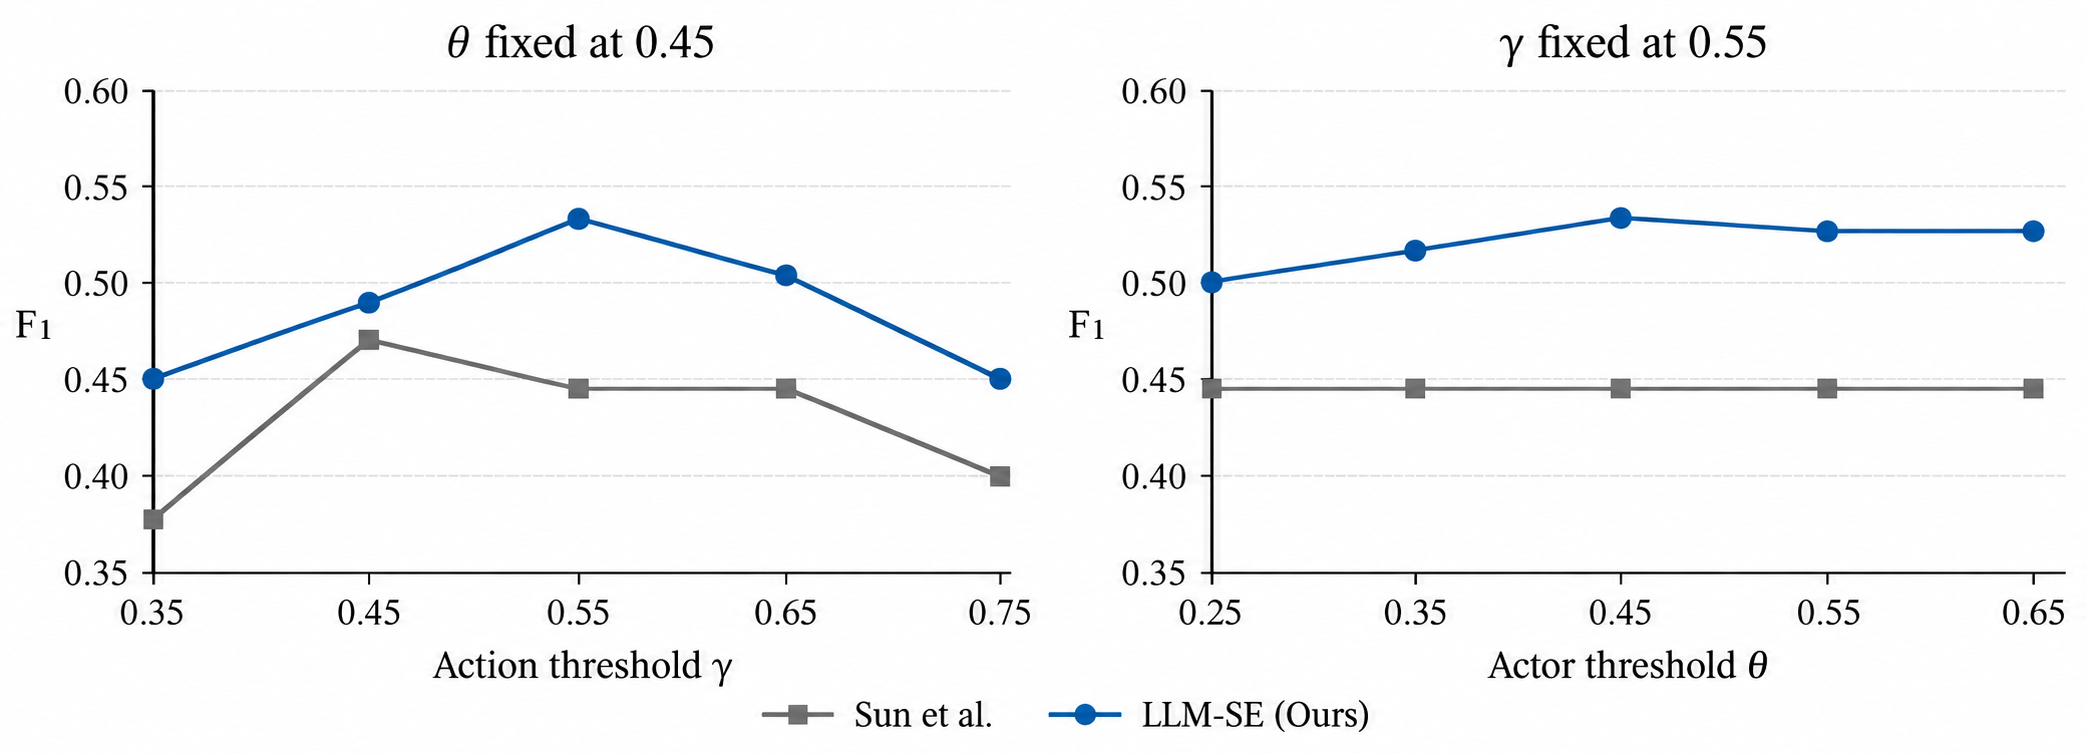
\includegraphics[width=\columnwidth]{fig3.png}
    \caption{Effects of action and actor similarity thresholds on compliance-checking F1.}
    \label{fig:threshold_sensitivity}
\end{figure}

\begin{table}[t]
\centering
\caption{Comparison of compliance-checking performance.}
\label{tab:downstream_results}
\begin{tabular}{lccc}
\toprule
\textbf{Method} & \textbf{Precision} & \textbf{Recall} & \textbf{F1} \\
\midrule
Sun et al. & 0.3814 & 0.5362 & 0.4458 \\
Winter et al. & \textbf{0.4634} & 0.5507 & 0.5033 \\
LLM-SE (Ours) & 0.4393 & \textbf{0.6812} & \textbf{0.5341} \\
\bottomrule
\end{tabular}
\end{table}

\textbf{Threshold Sensitivity.}
Fig.~\ref{fig:threshold_sensitivity} examines the effects of action ($\gamma$) and actor ($\theta$) similarity thresholds on compliance-checking F1. With $\theta=0.45$, LLM-SE reaches its highest F1 of 0.5341 at $\gamma=0.55$, while Sun et al. peaks at 0.4706 at $\gamma=0.45$. LLM-SE outperforms Sun et al. across all tested values of $\gamma$. With $\gamma=0.55$, LLM-SE performs best at $\theta=0.45$, while Sun et al. remains unaffected by $\theta$.

\textbf{Performance Comparison.}
On the GDPR-based benchmark (Table~\ref{tab:downstream_results}), LLM-SE achieves an F1 of 0.5341 versus 0.4458 for Sun et al. under shared thresholds, an improvement of 8.83 percentage points. It also outperforms Winter et al. (0.5033) by 3.08 percentage points. LLM-SE achieves the highest recall (0.6812), while Winter et al. achieves the highest precision (0.4634). 
This suggests that improved semantic extraction benefits downstream compliance checking.

Despite these improvements, LLM-SE still produces false-positive violations. Accurate semantic extraction alone does not guarantee reliable matching between regulatory requirements and BPMN process elements, which remains a challenge.

\section{Conclusion}
\label{sec:5}

We propose LLM-SE for design-time business process compliance checking. It combines prompt-based extraction with deterministic post-processing to construct Rule Records containing six regulatory semantic elements, reducing reliance on manually designed extraction rules and lexical resources. These records support compliance checking against BPMN process models.

On EStG-150, LLM-SE improves Overall Micro-F1 from 0.763 to 0.838 compared with the Sun-based method. Prompt analysis shows consistent benefits from semantic examples, while additional instructions do not always improve performance. On the GDPR-based development benchmark, LLM-SE achieves a checking F1 of 0.5341, outperforming the evaluated Sun and Winter baselines. However, reliable matching between regulatory semantics and BPMN process elements remains challenging. Future work will improve this matching and evaluate the approach on independent datasets.

\section*{Acknowledgment}

This work is partially supported by the Hunan Provincial Natural Science
Foundation of China under Grant No: 2026JJ50519.
\textit{Guosheng Kang} is the corresponding author.

\bibliographystyle{IEEEtran}
\bibliography{reference}

\end{document}